% file: 3-6-graph-decomposition/bicomponent-example-bicomponents.tex

\documentclass[tikz]{standalone}
\usetikzlibrary{positioning}

\begin{document}
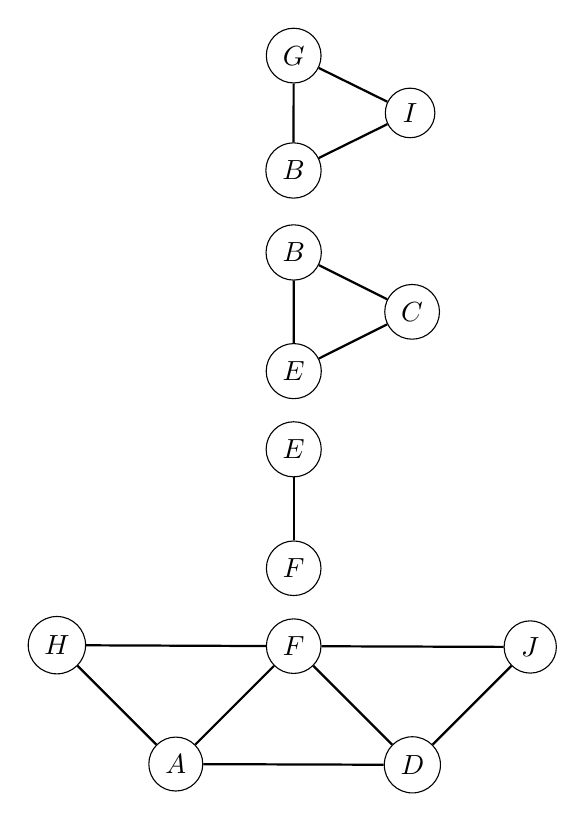
\begin{tikzpicture}[every node/.style = {draw, circle, minimum size = 6pt},
  node distance = 0.25cm and 1.0cm,
  every edge/.style = {draw, thick}]
  \begin{scope}
    \node (g) {$G$};
    \node (i) [below right = of g] {$I$};
    \node (b) [below left = of i] {$B$};

    \path (g) edge (b)
	      edge (i)
	  (b) edge (i);
  \end{scope}

  \begin{scope}[yshift = -2.5cm]
    \node (b) {$B$};
    \node (c) [below right = of b] {$C$};
    \node (e) [below left = of c] {$E$};

    \path (b) edge (e)
  	      edge (c)
  	  (c) edge (e);
  \end{scope}

  \begin{scope}[yshift = -5.0cm]
    \node (e) {$E$};
    \node (f) [below = 0.8cm of e] {$F$};

    \path (e) edge (f);
  \end{scope}

  \begin{scope}[yshift = -7.5cm, node distance = 1.0cm and 1.0cm]
    \node (f) {$F$};
    \node (a) [below left = of f] {$A$};
    \node (d) [below right = of f] {$D$};
    \node (h) [above left = of a] {$H$};
    \node (j) [above right = of d] {$J$};

  \path (f) edge (h)
	    edge (a)
	    edge (d)
	(h) edge (a)
	(a) edge (d)
	(d) edge (j)
	(j) edge (f);
  \end{scope}
\end{tikzpicture}
\end{document}
